\documentclass[licencjacka,en]{pracamgr}

% Authors
\autor{Marcin Chrzanowski}{370754}
\autori{Jakub Sarzyński}{371676}
\autorii{Agnieszka Świetlik}{371819}
\autoriii{Mikołaj Walczak}{371852}

% Metadata
\title{LAMP stack for Kubernetes}
\titlepl{LAMP stack dla Kubernetesa}
\kierunek{Computer Science}
% Supervisor
\opiekun{dr Janina Mincer-Daszkiewicz,\\ Instytut Informatyki}


\date{June 2018}
\dziedzina{TODO: Socrates-Erasmus classification}
\klasyfikacja{TODO: ACM Computer Science classification}

% Keywords
\keywords{Kubernetes, Custom Resources, MySQL, PHP, Apache, Cluster}

\usepackage[backend=biber]{biblatex}
\addbibresource{references.bib}
\usepackage{hyperref}
% \usepackage{titlesec}
\setcounter{secnumdepth}{3}
\usepackage{graphicx}
\usepackage{listings}
\lstset{
    basicstyle={\ttfamily}
}

\begin{document}
  \maketitle

  \begin{abstract}
  This project’s purpose was to provide a convenient way to set up a LAMP 
  stack on Kubernetes. We focused on implementing the most complex layer 
  --- a MySQL operator to facilitate the creation of a cluster of replicated 
  MySQL databases. In this dissertation we present a detailed description of 
  the design and implementation of the project. 
  \end{abstract}

  \tableofcontents

  \chapter{Introduction}
In the fast-paced world of modern web technologies, services are expected to
efficiently and reliably process large amounts of data. As such, developers
and system administrators want to create systems that are scalable. Scalability,
while desirable, is an issue that significantly adds to the complexity of
problems faced by software engineers every day. This has led to the emergence of
technologies that orchestrate entire clusters, providing automatization that
makes managing such systems easier.

\textbf{Kubernetes} is an open-source container orchestrator developed by
Google. It is used by leading tech companies to automate the deployment,
scaling, and management of their applications~\cite{kube-usecase}. Its common
use cases are cloud computing systems and microservices-oriented architectures.

The main feature provided by Kubernetes and similar orchestration
systems is the management of containerized applications. Containers are
a~lightweight and portable alternative to virtual machines. In recent years,
the~advantages of containerization have been recognised, which has led to
the~rapid development of supporting technologies, such as Docker or rkt.

A central part of many web applications is a~performant database. Despite
the~variety of new database engines constantly appearing on the market, many
developers still decide to rely on \textbf{MySQL}. According to the db-engines
statistics~\cite{db-eng}, MySQL is the second most used database
engine.

Our project is focused on developing tools for setting up and managing
a~\textbf{LAMP}\footnote{Linux host with Apache web server, MySQL database,
and PHP as the server-side programming language.} stack in Kubernetes. Our main goal is to
extend the Kubernetes API with options for MySQL database
management and provide users with a user-friendly command line tool. As
a~result, developers should be able to more effortlessly benefit from
Kubernetes’ advantages, such as scalability. Leveraging the powerful
abstraction system provided by Kubernetes in such a way will remove
much of the complexity traditionally caused by the database layer of
an~application.

There are existing unofficial tools with similar functionalities for various
databases and systems. Vitess~\cite{vitess} is an~open source
clustering system for MySQL databases that can interface with
Kubernetes. We are aiming for a simpler solution that utilizes
Kubernetes' native method of extending its API ---
\textbf{CustomResourceDefinitions}. Another existing tool,
the Crunchy Data PostgreSQL Operator~\cite{psql-op}, is closer in scope to what we want to
accomplish, providing a CustomResourceDefinition for Postgres databases.

This dissertation is divided into eight chapters. We start with the necessary 
preliminary knowledge about Kubernetes and custom resources. Next, we cover 
our workflow and development stack. The main chapter describes the design and 
implementation details of the MySQL Operator's functionalities. The following 
chapter covers the command line interface we  provided to facilitate the usage
of our tools. The final sections explain main  design decisions, obstacles encountered,
and future considerations for further work on the project.

We collaborated closely as a team on both the MySQL Operator as well as this
dissertation. All design decisions were discussed between the four of us and
agreed upon by consensus. Marcin Chrzanowski was mostly responsible for
implementing the MySQLCluster operator's functionalities. Jakub Sarzyński
created most of the command line interface. Agnieszka Świetlik was responsible
for implementing the backup system. Mikołaj Walczak took on an unofficial tech
lead role and was also in charge of setting up our development infrastructure.
He administrated the Continuous Integration system, managed software
dependencies, and set up testing, in addition to contributing code to various
areas of the project.

  \chapter{Background}

\section{Kubernetes}
\section{Custom Resource Definition}

  \chapter{Development Stack}

In this chapter we provide the general overview of our workflow and
development stack.

\section{Version Control System}
Our version control system of choice is Git and we host our repository on
GitHub~\footnote{https://github.com}. Being the most popular git host,
GitHub is well integrated  with many developer tools such as Golang’s
\texttt{go get} and various continuous integration systems. On top of that,
we use common GitHub features for managing current tasks and project development.

\subsection{Workflow}
We follow a fairly standard git workflow. New features are developed on 
separate branches, branched directly off of \texttt{master}. Once the code
is ready, the branch is pushed to our central GitHub repository and code 
review is requested from other team members. After positive feedback from 
the CI system and two approvals, the pull request is merged to the 
\texttt{master} branch. To retain a linear git history, all feature branches 
are rebased onto the \texttt{master} branch before merging.

\section{Continuous integration}

\subsection{Travis}
Travis CI~\cite{travis} is a hosted continuous integration service with
a free option for open source projects.
Unlike many other services, it does not require server-side 
configuration, but relies only on .travis.yml files placed inside 
the project's source directory. This makes it easy to have different test 
code per branch and removes the necessity to manage permissions separately 
for the repository and for the CI system. Travis integrates well with other 
tools used in our project (GitHub and Slack).

Along with Travis CI, we have 
decided to use Coveralls~\cite{coveralls} --- a web service that 
tracks code coverage\footnote{the percentage of the source code of a~program 
is executed when a particular test suite runs} over time, and ensures that 
all new code is fully covered by tests.

\subsection{Kubernetes Cluster}
To perform integration tests during the continuous integration process we 
used Minikube~\cite{minikube} --- a lightweight
Kubernetes implementation that creates a VM on the local machine and deploys 
a simple cluster containing only one node.

\subsection{Continuous Deployment}
The Docker image built from the \texttt{master} branch is automatically 
deployed to DockerHub~\cite{docker}. This way users can download
and use our project easily as a docker image. Each stable version of our 
project is manually added and reflects a specific git commit.

\section{Communication}
As our communication tool, we have chosen Slack~\cite{slack} --- 
a modern IRC-like communicator. Slack features persistent chat rooms
(channels) organized by topic, comes with a large number of third-party 
services, and supports community-built integrations.

  \chapter{MySQL Operator}

In this chapter the main part of the project is described. First we provide 
a high-level overview, followed by a detailed design of the MySQL Operator 
and Backup custom resources. Next, we present basic usage examples.

\section{High-level overview}
MySQL Operator allows a user to easily deploy replicated MySQL databases on a Kubernetes cluster.
It provides single-command cluster creation, scaling and backup scheduling. The project is divided
into two essential parts:
\begin{itemize}
	\item The actual operator --- a running service which listens for changes on custom resource
	objects and creates a new desired configuration on the Kubernetes cluster.
	\item A command line interface --- an optional tool facilitating interaction with the created
	resources.
\end{itemize}

In this chapter we will focus on the first one of mentioned elements.

\subsection{Functionalities}
The MySQL Operator allows the user to create, delete, update, backup and restore MySQL clusters.

When \textit{creating} the cluster, the operator deploys a new instance of a replicated MySQL
database cluster alongside with all additional Kubernetes objects necessary for a proper deployment.
Additionally, rather than initializing a fresh cluster, data may be \textit{restored} from a backup file.

When a cluster is to be removed, the operator takes care to delete the cluster and its
configuration from Kubernetes. Unless explicitly specified, database data remains available, to be
cleaned up manually.

A running cluster may be \textit{updated} by, for example, changing the configuration (port,
password) or scaling the cluster (increasing or decreasing the number of replicas deployed in the
cluster). When such an update is requested, the operator makes sure all the relevant Kubernetes
objects are updated to reflect the new cluster configuration.

We provided users with the ability to schedule backups. \textit{Scheduling a backup} initiates a
recurring backup. The backup job’s behavior is similar to a cron job’s --- backups are created
cyclically at regular intervals.

\section{Project Design}

\subsection{Custom Resource Definition design}
The main custom resource provided by our project is \textbf{MySQLCluster}. A custom resource of this kind
represents a cluster of replicated MySQL servers. It has a unique name specified by the user and
that name also becomes the name of a Kubernetes Service through which the database is exposed.
Another custom resource defined in our project is \textbf{MySQLBackup}. Objects of this kind are created when
the user wants to schedule database backups. Each instance of this resource corresponds to a backup
schedule request for a specific cluster.

\subsection{Design Patterns}
The MySQL Operator’s implementation is primarily based on two common Kubernetes design patterns:
the controller and operator patterns. A \textbf{controller} is an informer whose responsibility is
to monitor changes in an application’s state. On each change, a predefined controller function is
executed. An \textbf{operator} builds on ideas from the controller pattern and basic Kubernetes
concepts. It is responsible for creating, configuring and managing stateful applications running on
clusters. Operators extend the Kubernetes API and create multiple instances of applications like
core Kubernetes resources.

\begin{figure}[!ht]
    \centering
    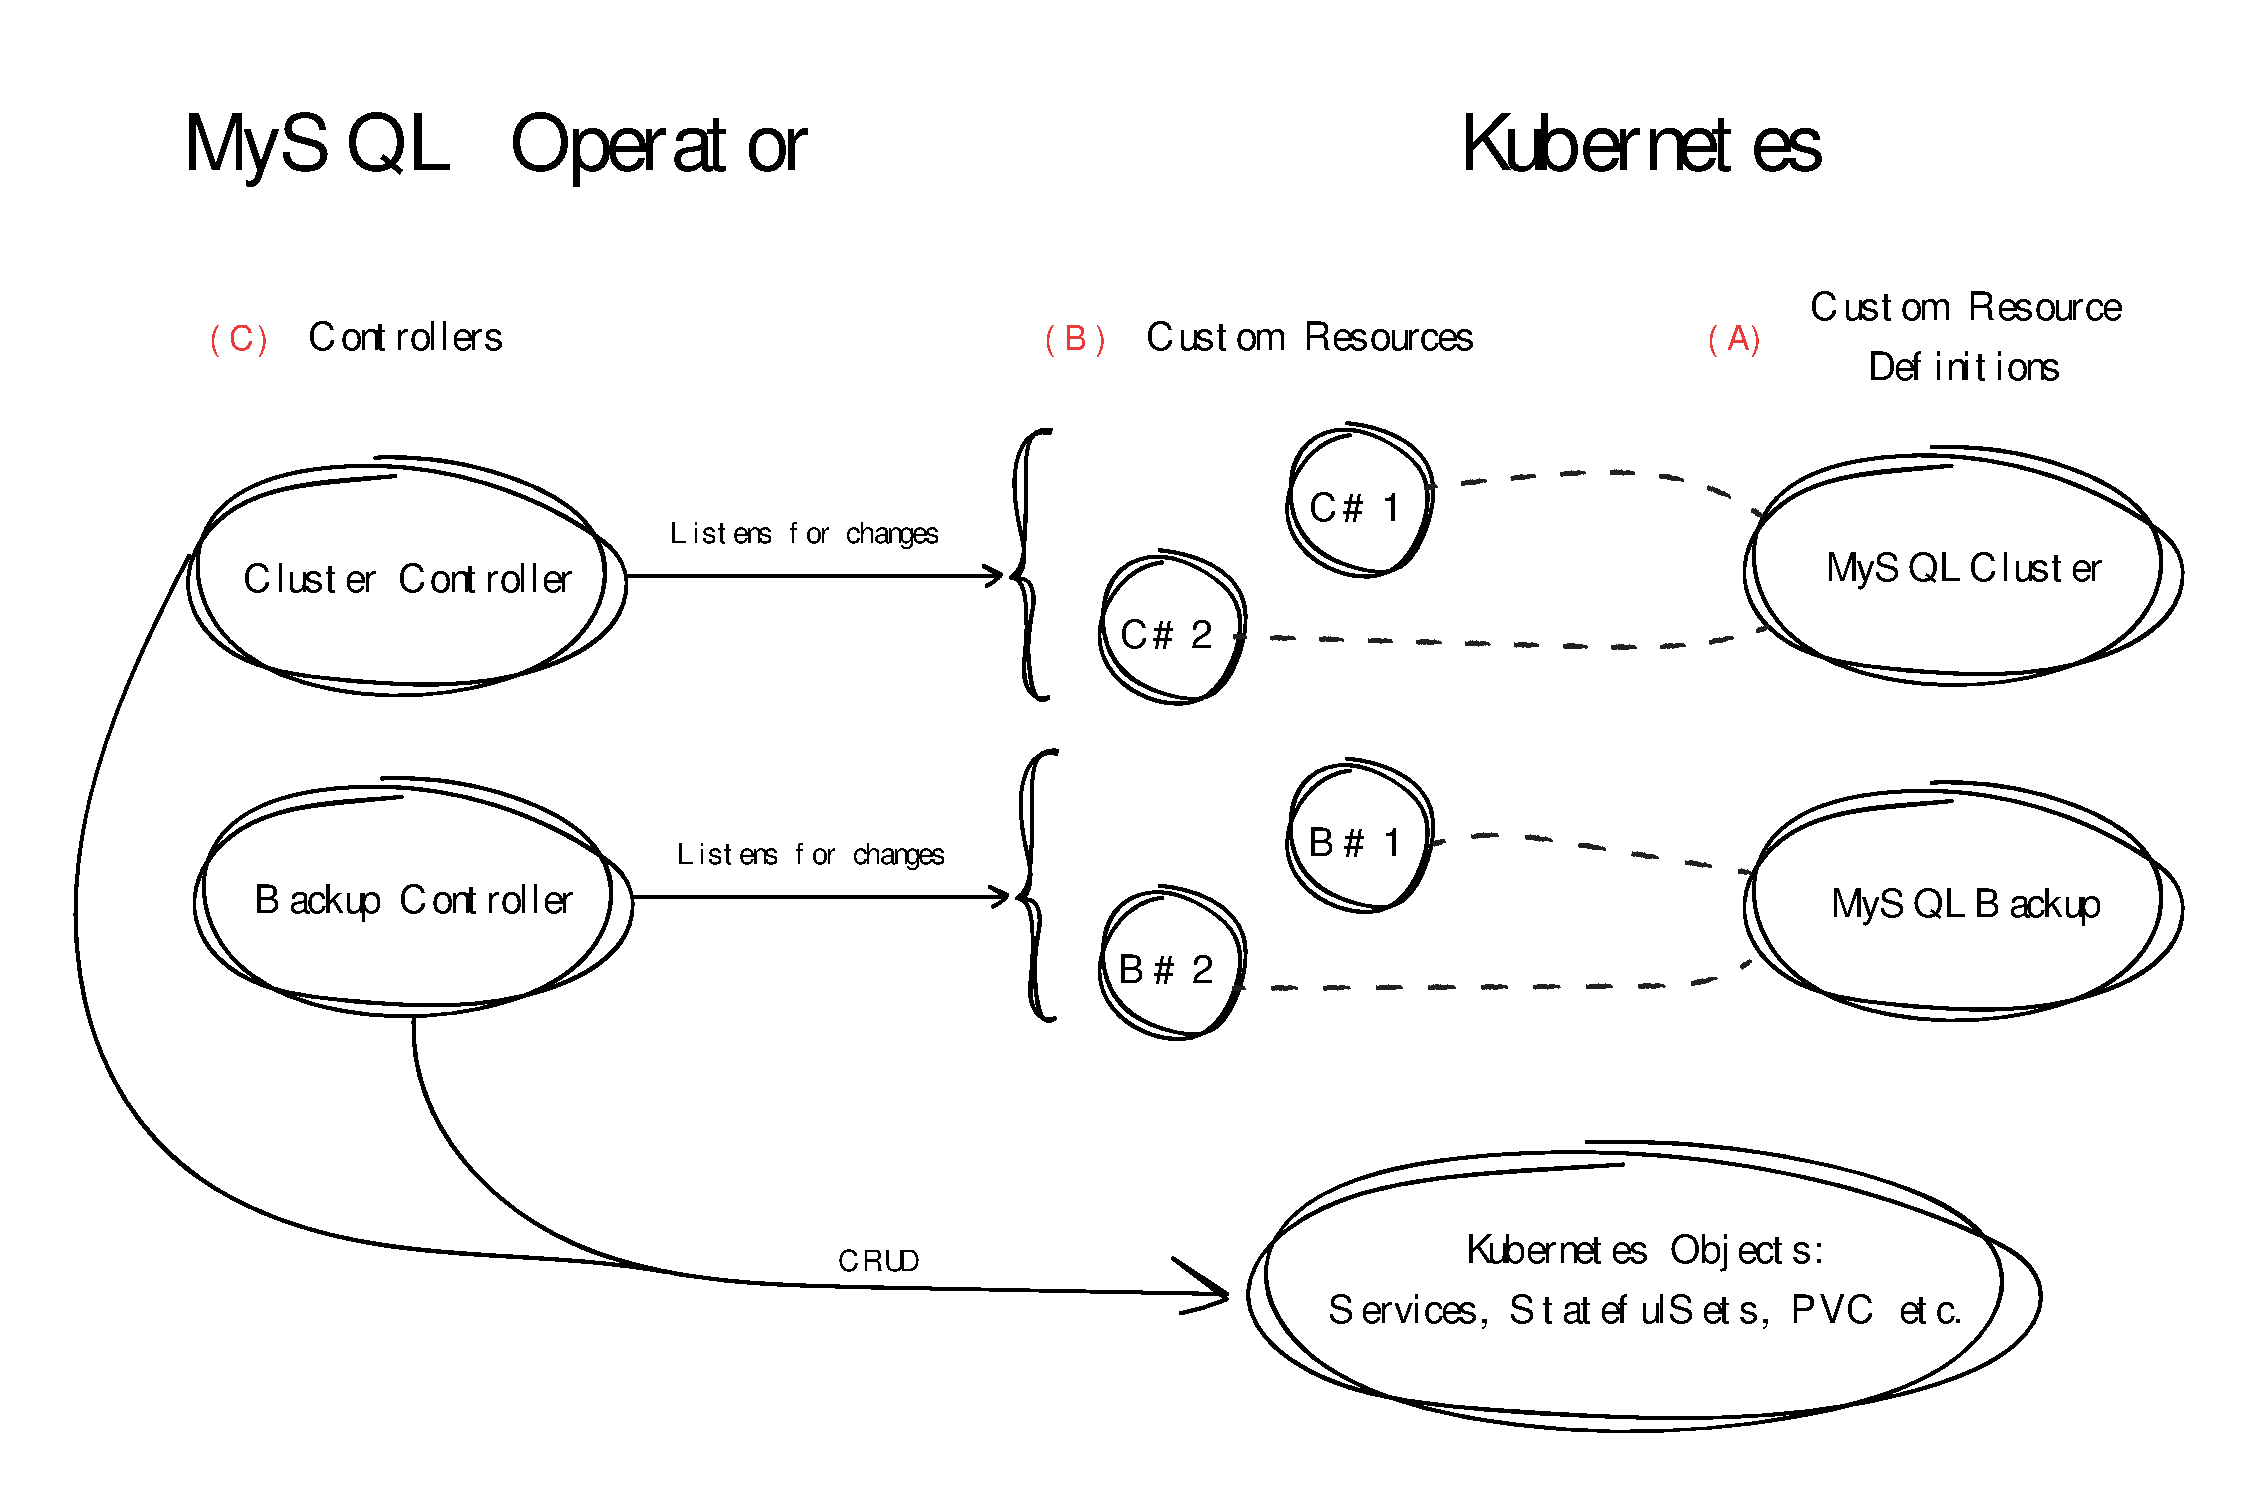
\includegraphics[width=1\textwidth, angle=0]{img/Design.pdf}
    \caption{MySQL operator architecture}
    \label{fig:design}
\end{figure}

To get a better understanding of the controller and operator design patterns, let’s look at an
example of how an operator will respond to a user’s action. Let’s say the user wants to modify a
MySQLCluster instance. From the user’s point of view, this can be done by issuing a
\texttt{kubectl patch} command. From the operator’s point of view, an \textbf{Update} event is
received and the corresponding operator handler is called by the controller.

We use the controller and operator patterns to manage resources related to both 
MySQL servers and backup jobs. A high level overview of the project design is
illustrated in Figure \ref{fig:design}. During operator startup, two
CustomResourceDefinitions (figure \ref{fig:design} A) are registered into the Kubernetes API.
From this point on, users can define their own custom resource instances (Figure \ref{fig:design} B) ---
MySQLClusters (ex. C1, C2) and MySQLBackupSchedules (ex. B1, B2). Each kind of
custom resource has its corresponding controller listening and reacting to changes on these
resources. The cluster controller and the backup controller (Figure \ref{fig:design} C), though technically
goroutines\footnote{Function or methods that run parallel with other functions or methods.} in a single
MySQL Operator process, can be thought of as separate processes responsible for separate parts of the
cluster’s architecture. Thanks to these constructs we can monitor custom resource instances and adjust
all the related objects as necessary. The operator pattern was designed for stateful applications, making
it suitable for both database cluster and backup management.~\cite{coreos}

\subsection{Detailed design of the MySQL cluster}

\subsubsection*{Create}
The internal implementation of a MySQLCluster within Kubernetes consists of two parts. First,
several Pods (one for each replica) running a containerized MySQL server are managed by a
StatefulSet. Secondly, two Kubernetes Services expose the MySQL servers as named endpoints by
configuring Kubernetes’ DNS. Two distinct Services are necessary because different nodes in the
cluster have different capabilities. Specifically, the master node is the only one to which writing
is allowed. Therefore, one Service exposes only the  master node and allows for both reading and
writing, while the second Service connects to all nodes, but allows for read-only access. 

Our operator is responsible for creating the appropriate StatefulSet and Services when the user
creates a MySQLCluster object.

\subsubsection*{Services}
A Service object represents the network configuration necessary to expose a specific service at a
particular domain name and port. To expose the MySQLCluster we create what’s called a
“headless Service.” No specific IP address is configured. Instead, we specify which Pods (the ones
managed by our StatefulSet) should be available under the given address. The Service then configures
Kubernetes’s DNS to return an \textbf{A record}\footnote{An \textbf{A record} maps a domain name to
the IP address (IPv4) of the computer hosting the domain.} pointing at each of the Pods. This
essentially means that DNS load balancing is used to load balance queries to the database cluster.

\subsubsection*{Delete}
When a MySQLCluster instance is deleted, all the related objects should be cleared from Kubernetes
as well. Thanks to the \texttt{ownerReferences} attribute, we do not have to worry about manual
deletion of dependent structures. Kubernetes understands that some objects are owned by others, and
when a parent object is deleted, the children will be deleted as well. Thus all we have to do is to set
the \texttt{ownerReferences} field of the Services and StatefulSet we create to the parent
MySQLCluster object’s UID and Kubernetes will take care of garbage collection for us.

Objects which are meant to have a longer lifetime, such as PersistentVolumeClaims and the
PersistentVolumes on which database data is stored, will not be deleted. In order to
proceed with a hard delete, these constructs have to be removed separately.

\subsubsection*{Scale/Update}
The operator’s update handler receives information about how the cluster’s configuration looked
like before the update, and what the new requested configuration is. Based on this, we can create
new configurations for the cluster’s related objects (the Services and StatefulSet) and issue update
requests for those. In case of an error, we update the MySQLCluster’s status field with an error
message. The cluster might be partially updated and its previous state is not reinstated.

\begin{figure}[!ht]
    \centering
    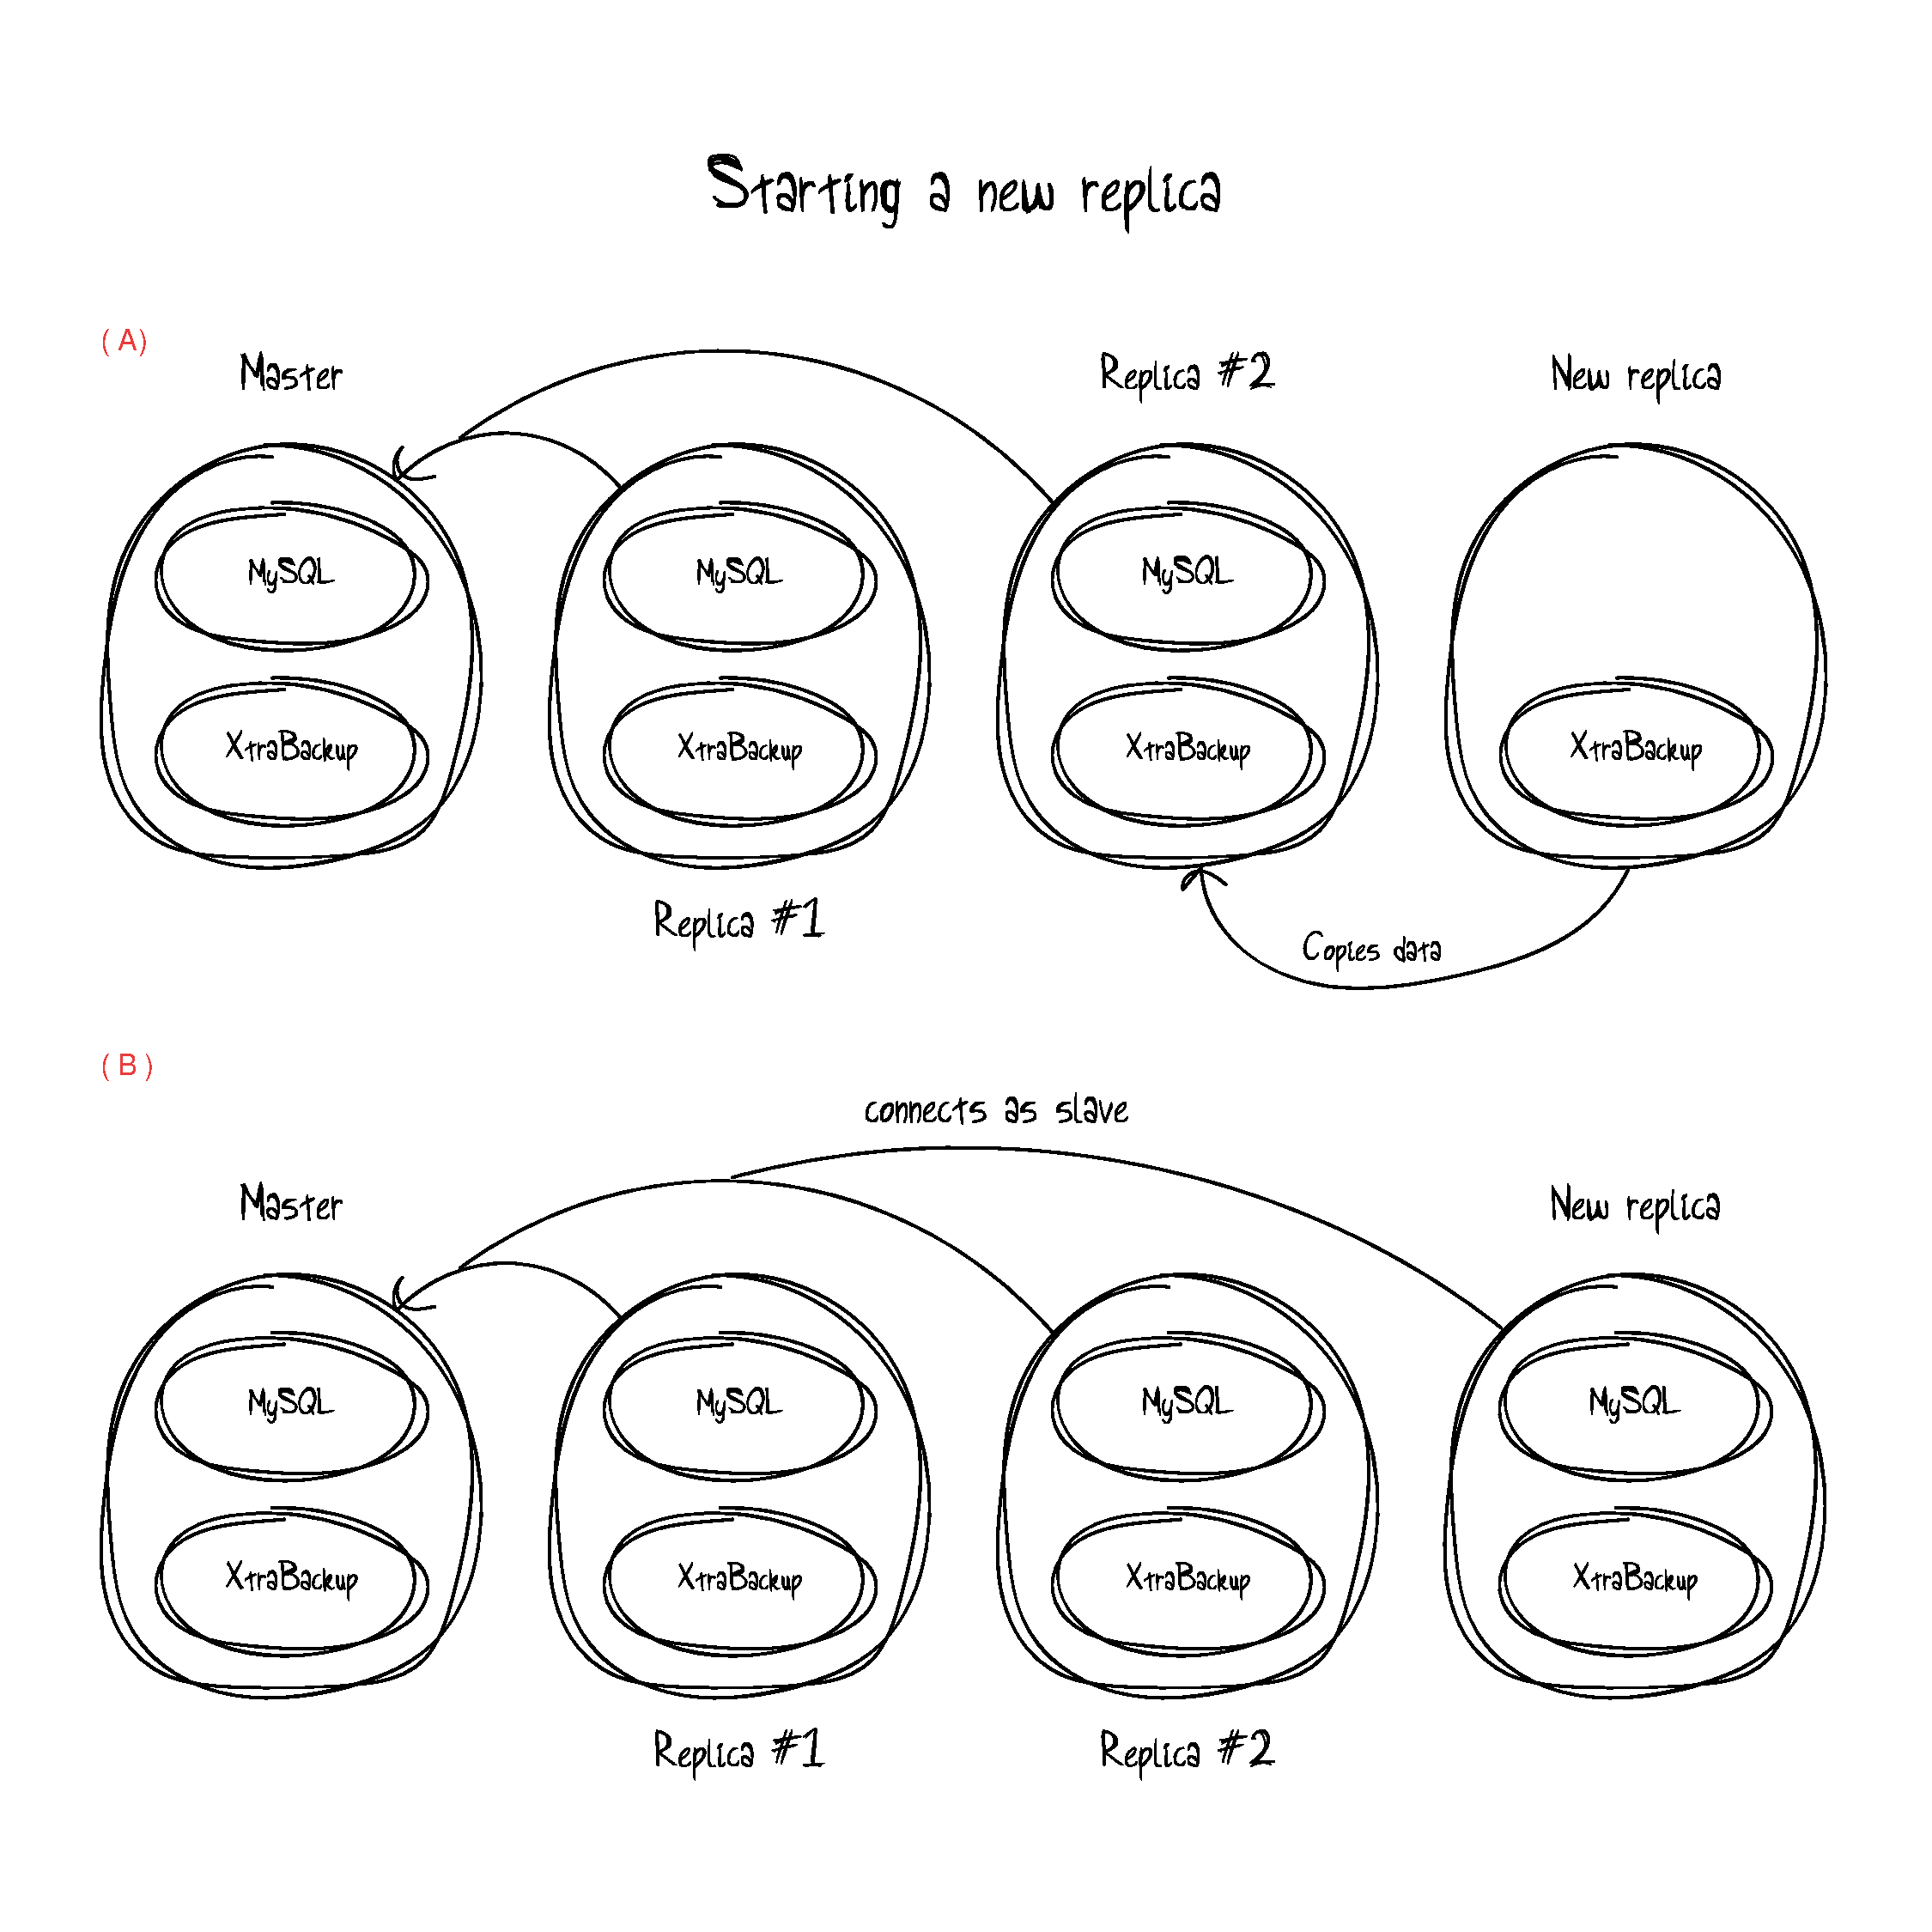
\includegraphics[width=1\textwidth, angle=0]{img/replication.pdf}
    \caption{Replication}
    \label{fig:replication}
\end{figure}

Core Kubernetes structures, such as StatefulSets or Services, are already equipped with mechanisms
for scaling and configuration updates that do most of the work for us (for example, starting up new
Pods if the replica count is increased). However, when scaling up, we need to copy the cluster’s
data to the newly created replicas. To achieve non-blocking replication, every pod has an XtraBackup
container running beside the main MySQL server container. \textbf{Percona XtraBackup}~\cite{percona}
is a popular, lightweight, and easy to use program that replicates data from a database without
stopping it. When a new Pod in a StatefulSet is created, its initial data is copied from the
previous Pod by connecting to its XtraBackup (exposed via ncat\footnote{Tool to read from and
write to network connections using UDP or TCP.}) --- each new replica copies the data from its direct
predecessor (Figure \ref{fig:replication} A). This allows us to avoid overloading the master node,
which would have occurred if the replica nodes all copied data from it. A new replica is then connected
as a slave to the master MySQL server (Figure \ref{fig:replication} B).

\section{Detailed design of the MySQL backups}

\begin{figure}[!ht]
    \centering
    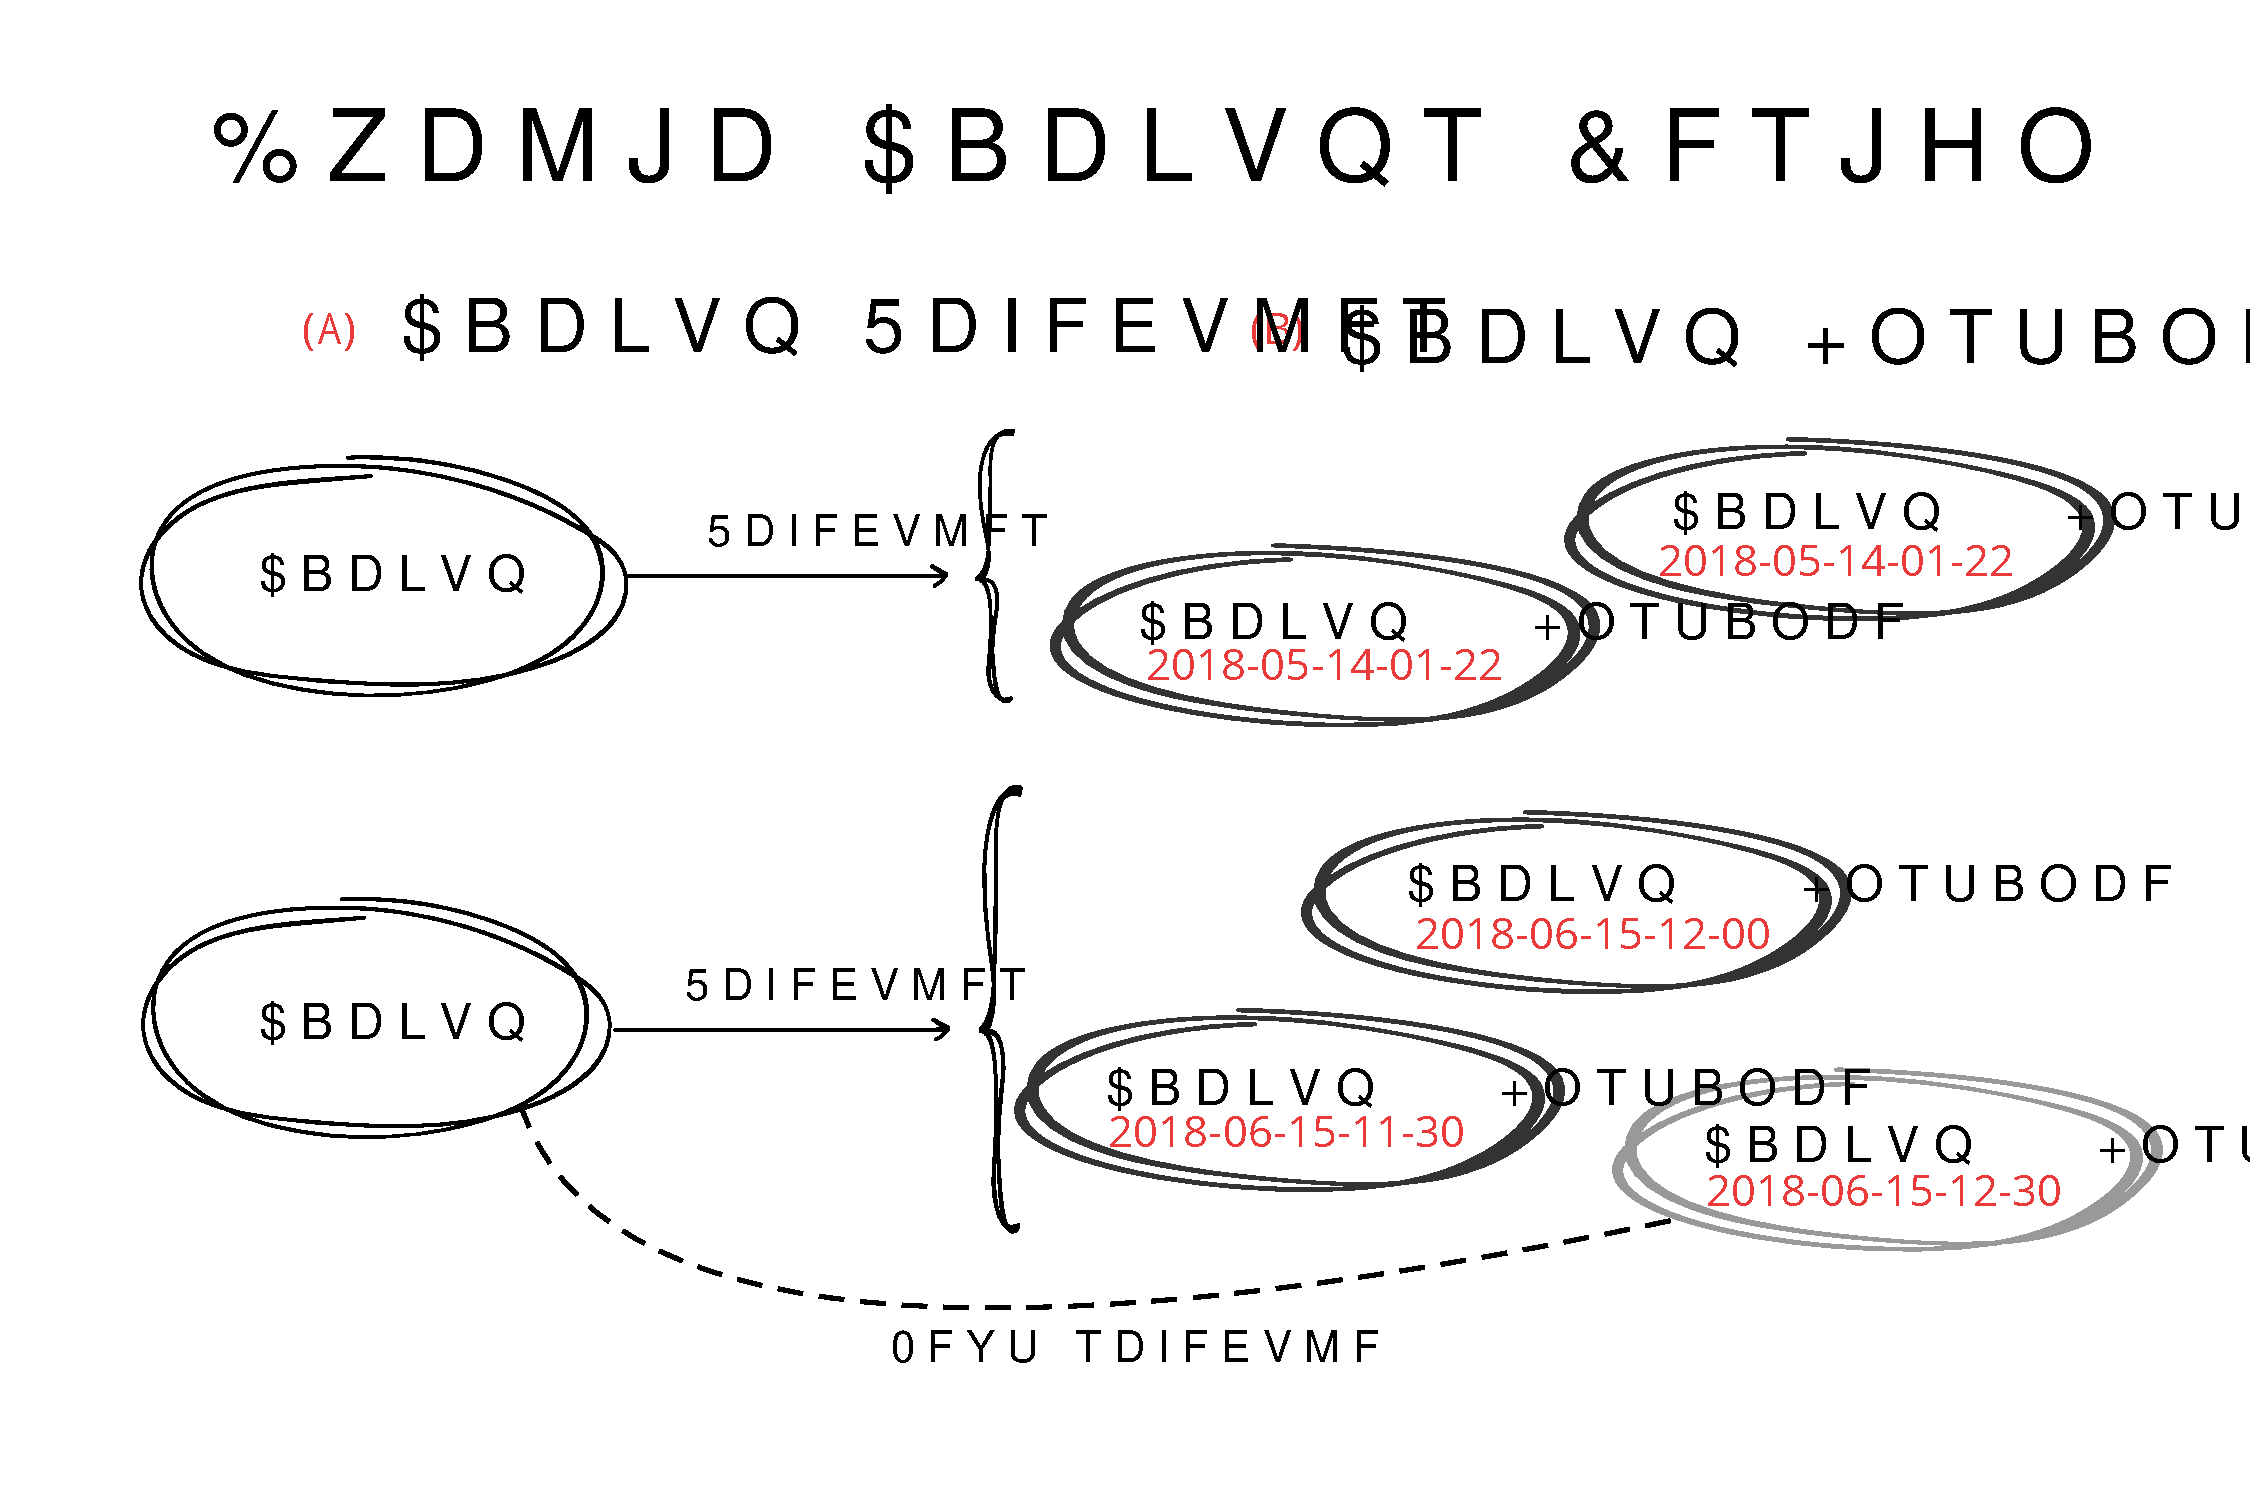
\includegraphics[width=1\textwidth, angle=0]{img/cyclic_backups.pdf}
    \caption{MySQL backup design}
    \label{fig:backups}
\end{figure}

\subsubsection*{Backup}
In order to provide users with cyclic backups of a MySQL cluster, we created 
two separate CustomResourceDefinitions: \textbf{MySQLBackupSchedule} and 
\textbf{MySQLBackupInstance}. Objects of the first type are responsible for 
scheduling and managing the groups of backups. At the same time, objects 
of the latter type reflect the actual backups created. As a result, each 
of the MySQLBackupSchedules can have multiple corresponding 
MySQLBackupInstances --- one for each backup created.

To gain a better understanding of this structure, let’s analyse the Figure 
\ref{fig:backups}. From the user point of view, cyclic backups are requested 
by creating a MySQLBackupSchedule object (A). Backup creation is handled 
by a Kubernetes CronJob object created by our operator. A CronJob periodically 
creates Kubernetes jobs which run to completion. In our case, each of these 
jobs creates a separate MySQLBackupInstance object (B). After that, the 
dedicated operator creates an actual backup without overwriting previous 
backups. The status of a MySQLBackupInstance object reflects the state of 
an actual backup --- the user can see if certain backup succeed. Thanks 
to this design it is also fairly easy to list all the existing backups, 
it’s simply listing the MySQLBackupInstance objects.

All the backups for a single MySQLBackupSchedule are stored in a single 
PersistentVolume. The backed up data is not deleted when the cron job is 
cancelled since PersistentVolumes are not owned by our object.

For the actual backup creation we reuse the solution applied for scaling 
up MySQL clusters. The backup mechanism utilizes the same XtraBackup endpoints 
to get the data from our database. Backups are always based on the master 
node’s data.


\subsubsection*{Restore}
Users can restore any backup instance from a chosen backup schedule. This is simply done by creating
a new MySQLCluster object with the name of the backup to restore from specified in the
configuration.

\section{Use Cases}
In order for the custom resources to be properly processed and an actual MySQL cluster deployed, a
running instance of the MySQL Operator is required inside the Kubernetes infrastructure. The
recommended option is to start a MySQL Operator image as a Deployment in the cluster:

\texttt{kubectl run mysql-operator --image=grtl/mysql-operator:latest}

\subsection{Cluster}
\subsubsection*{Create/Restore}

The MySQLCluster creation is the most essential part of the 
workflow. At this point user has to decide on cluster configuration.

\lstset{emph={"password", my-password}, emphstyle=\itshape}
\begin{lstlisting}
> kubectl create secret generic my-password \
	--from-literal=password="password"}

> kubectl apply -f cluster-config.yaml
\end{lstlisting}

\paragraph{Data to specify}
\begin{enumerate}
	\item Cluster name.\footnote{Cluster name must be unique, it will be the future reference
	to the cluster.}
	\item Root password \textit{(Kubernetes secret)}.
	\item MySQL port \textit{(optional, defaults to 3306)}.
	\item Number of replicas \textit{(optional, default to 2)}.
	\item Storage size \textit{(optional, default to 1Gi)}.
	\item Custom mysql image. \textit{(optional)}.
	\item Backup name \textit{(optional)}.\footnote{If provided, initial cluster data is restored
	from backup.}
\end{enumerate}

\paragraph{Example \textbf{cluster-config.yaml}}
\lstset{emph={"my-cluster", "my-password"}, emphstyle=\itshape}
\begin{lstlisting}[caption=cluster-config.yaml,captionpos=b]
apiVersion: cr.mysqloperator.grtl.github.com/v1
kind: MySQLCluster
metadata:
  name: "my-cluster"
spec:
  name: "my-cluster"
  password: "my-password"
  port: 3306
  storage: 1Gi
  mysqlImage: "mysql:latest"
  restoreFrom: 
	backupName: "my-backup"
	instance: "2017-12-14-01-22"
\end{lstlisting}

\subsubsection*{Delete}

It is possible to delete many clusters at the same time by simply writing
names of all the clusters we want to remove from Kubernetes.

\begin{lstlisting}
> kubectl delete mysqlcluster my-cluster
OR
> kubectl delete mc my-cluster
\end{lstlisting}

\paragraph{Data to specify}
\begin{enumerate}
	\item Cluster name \textit{(one or more)}.
	\item Persistent Volume Claims \textit{(optional)}.
\end{enumerate}

\subsubsection*{Update}

Not every element of configuration can be updated. Even though we aimed 
to provide the best configurability possible, users cannot modify the
cluster name.

\begin{lstlisting}
> kubectl apply -f cluster-config.yaml
\end{lstlisting}

\paragraph{Data to specify}
\begin{enumerate}
	\item Cluster name.
	\item Root password \textit{(Kubernetes secret, optional)}.
	\item MySQL port \textit{(optional)}.
	\item Number of replicas \textit{(optional)}.
\end{enumerate}

\subsection{Backup}
\subsubsection*{Create}

During the backup creation users specify how often they want their backups 
to be created.

\begin{lstlisting}
> kubectl create -f backup-config.yaml
\end{lstlisting}

\paragraph{Data to specify}
\begin{enumerate}
	\item Backup name \textit{(optional: defaults to auto generated based on cluster name)}.
	\item Cluster name.
	\item Time \textit{(CRON style, required)}.
	\item Storage \textit{(optional: default to the Cluster storage size)}.
\end{enumerate}

\noindent  \textbf{Additional info}

\noindent Database will be backed up in an automatically claimed Persistent Volume with the size
calculated based on the cluster current database size.

\paragraph{Example \textbf{backup-config.yaml}}
\begin{lstlisting}[caption=backup-config.yaml,captionpos=b]
apiVersion: cr.mysqlbackup.grtl.github.com/v1
kind: MySQLBackupSchedule
metadata:
  name: "my-backup"
spec:
  cluster: "my-cluster"
  time: "59 23 31 DEC Fri *"
  storage: 1Gi
\end{lstlisting}

\noindent  \textbf{Getting backup instances}

\noindent For getting created backup instances with a valuable output we recommend
using output flag with the following configuration:

\begin{lstlisting}
kubectl get mbi -o custom-columns="NAME:metadata.name,\
	STATUS:status.phase,SCHEDULE:spec.schedule,\
	CLUSTER:spec.cluster,CREATED:metadata.creationTimestamp"
\end{lstlisting}

\noindent Sample output:
\begin{lstlisting}
NAME          STATUS    SCHEDULE  CLUSTER    CREATED
bckp-instance Completed bckp      my-cluster 2018-04-27T14:42:33Z
\end{lstlisting}

\subsubsection*{Delete}

Deletion of the backups works in the same way as the cluster deletion.

\begin{lstlisting}
> kubectl delete mysqlbackupschedule my-backup
OR
> kubectl delete mbs my-backup
\end{lstlisting}

\paragraph{Data to specify}
\begin{enumerate}
	\item Cluster name \textit{(one or more)}.
	\item Persistent Volume Claims \textit{(optional)}.
\end{enumerate}

\subsubsection*{Update}

For backups the only value users can update is the backup 
scheduling time.

\begin{lstlisting}
> kubectl apply -f backup-config.yaml
\end{lstlisting}

\paragraph{Data to specify}
\begin{enumerate}
	\item Time \textit{CRON style}.
\end{enumerate}

  \chapter{Command Line Tool}
In this chapter we describe \texttt{msp} --- a command line tool we created
to facilitate usage of the MySQL Operator. First, we explain the basic CLI
concept, followed by a description of technologies used, and finally a
detailed description of the functionalities provided by our tool. We also
provide a few usage examples to outline the most common use cases.

\section{CLI Basics}
\texttt{msp} provides a layer of abstraction over management of MySQLCluster
and MySQLBackupSchedule objects. Rather than writing verbose yaml files and manually
modifying Kubernetes’ configuration via \texttt{kubectl}, a user can easily
perform most actions related to managing their MySQL cluster with a single
\texttt{msp} command. Additionally, a CLI tool like this helps inexperienced users
get started with our system, and allows Kubernetes system administrators to
write more concise and expressive automation scripts.

\section{Technologies}
Like the rest of our project, \texttt{msp} is written in Go. Our implementation
bases on Cobra~\cite{cobra} --- a framework for writing command line interfaces
similar to many UNIX shell programs. Cobra is widely used in the Go and
Kubernetes ecosystems, most prominently in \texttt{kubectl} itself. The
library is designed to facilitate the creation of easily extensible and
customizable CLI tools. Cobra programs are typically called with a list
of structured arguments specifying an object, an action to perform on the
selected object, and optionally a list of flags that customize the program’s
behavior.

\section{Functionalities}
The treelike command structure implies the natural order of the whole CLI
tool. Consequently, each command in our tool has the following form: \\
\centerline{\textit{msp resource-type action resource-name flags}}
\texttt{msp} can be used to create, update, or delete both MySQLClusters
and MySQLBackupSchedules. Flags can be global or local, referring
to resource types and actions. To set global options, needed for proper
functioning of the program, \texttt{msp} uses the following flags:
\begin{itemize}
    \item \texttt{kubeconfig} --- location of the kubeconfig file needed to
        establish a network connection with a Kubernetes cluster.
    \item \texttt{namespace} --- Kubernetes namespace in which resources will be created.
    \item \texttt{force} --- to ignore errors during cascade deleting.
\end{itemize}


\section{MySQL Operator Use-cases}

These use cases show most of the actions that can be performed to manage a cluster and its data.

\subsection{Cluster}

\subsubsection*{Create}
\noindent Creating a new cluster with an already exisiting Secret.

\begin{lstlisting}
> msp cluster create "my-cluster" --secret "my-secret"
\end{lstlisting}

\noindent Creating a new cluster along with defining a new Secret.

\begin{lstlisting}
> msp cluster create "my-cluster" --secret "my-secret" \
	--password "password"
\end{lstlisting}

\noindent Creating a new cluster from a backup instance.

\begin{lstlisting}
> msp cluster create "my-cluster" --backup "backup-name" \
	--instance "backup-instance"
\end{lstlisting}

\noindent Creating a new cluster with a specified port, image, storage, and number of replicas.

\begin{lstlisting}
> msp cluster create "my-cluster" --port 1337 --image mysql:img \
	--replicas 7 --secret "my-own-secret"
\end{lstlisting}

\subsubsection*{Delete}

\texttt{msp} provides users with more functionalities. Users can perform a hard
delete, removing not only the cluster but also all database information.

\noindent Deleting two clusters.

\begin{lstlisting}
> msp delete cluster "my-cluster" "my-cluster2"
\end{lstlisting}

\noindent Deleting a cluster along with PVC’s.

\begin{lstlisting}
> msp delete cluster "my-cluster" --remove-pvc
\end{lstlisting}

\subsubsection*{Update}
\noindent Updating a cluster with a new Secret, port, and number of replicas.

\begin{lstlisting}
> msp update cluster "my-cluster" --replicas 4 --port 1337 \
	--secret "my-new-secret"
\end{lstlisting}

\subsection{Backup}

\subsubsection*{Create}
\noindent Creating a backup schedule that creates a backup instance at 23:59 December 31 every year.

\begin{lstlisting}
> msp create backup --cluster "my-cluster" \
	--time "59 23 31 DEC Fri *"
\end{lstlisting}

\noindent Creating a backup schedule named "elite" in Kubernetes that creates
a backup instance at 13:37 every day. The 2Gi of storage is shared among
the backup instances.

\begin{lstlisting}
> msp create backup --name "elite" --cluster "my-cluster" \
	--time "13 37  *  *  * *" --storage 2Gi
\end{lstlisting}

\subsubsection*{Delete}
\noindent Deleting two backup schedules.

\begin{lstlisting}
> msp delete backup "my-backup" "my-backup2"
\end{lstlisting}

\noindent Deleting a backup schedule along with its PVC's.

\begin{lstlisting}
> msp delete backup "my-backup" --remove-pvc
\end{lstlisting}

\subsubsection*{Update}
\noindent Updating a backup schedule's time field.

\begin{lstlisting}
> msp update backup "my-backup" --time "12 20 * * * *"
\end{lstlisting}

  \chapter{Project decisions}
In this chapter we describe non trivial decisions made while designing the project, as well as the
reasons behind them.

\section{Backup}
Even though it is certain that we want to use Custom Resource Definitions, the question on how to
use them still remains. The main object in the project is MySQL Cluster, which can be added,
deleted, updated, scaled freely as a CRD instance. The remaining question is about backups.

We decided to use the operator pattern again for managing backups. In the case of the MySQL
operator it was fairly obvious what needed to be done to implement a cluster --- create a
StatefulSet to run servers, and a Service to expose them at one DNS endpoint. Designing a system
for backups required a bit more thought.

\section{Cyclic Backups}
The Kubernetes’ design philosophy proclaims that users should describe the desired state and
Kubernetes will try to adjust to this request. As mentioned in the Background chapter, Kubernetes 
objects are by convention meant to represent nouns, not verbs. Following this ideology, we 
decided to implement a cyclic backup creation. What is more, creating backups on a cyclic schedule 
is a good system administration practice. However, for the users’ convenience, single backups are 
also supported.

\section{Backup Schedules and Instances}
In order to implement cyclic backups, there must exist objects responsible for managing each one of
these repetitive actions. At the same time, we have to keep track of existing backups. Taking this
into account, we provide users with the MySQLBackupSchedule custom resource, whose meaning is not a
verb ("create a backup"), but a noun ("an agent that creates backups periodically"). At the same
time, another resource --- MySQLBackupInstance is created to allow us for monitoring existing
backups. 

\section{LAMP Stack}
LAMP stands for Linux, Apache, MySQL, and PHP, and refers to a stack of technologies commonly used
for hosting web services. Our project’s purpose was to provide a convenient way to set up a LAMP
stack on Kubernetes. We quickly realized that the only part of this stack that needed special
consideration was the database layer. An Apache server serving a simple PHP web application can
easily be deployed using a Kubernetes Deployment and a publicly available Apache Docker image.
Kubernetes Deployment objects were designed specifically for these kinds of stateless applications.
As such, we decided to focus our efforts on implementing the MySQL operator.

  \chapter{Obstacles}
In this chapter we describe the biggest difficulties we encountered while implementing our project,
and how we resolved them.

\section{High Entry Threshold}
Kubernetes is a fairly young project, but already highly advanced and complex. It is constantly
improving and changing. It is written in Go --- a programming language none of
us had used before starting work on this project. We had to get a good grasp of Kubernetes’
high-level philosophy, as well as dive deep into the detailed design of its objects and the
lower-level internals of how they are managed and manipulated. We had to wade through large amounts
of documentation (some of it freshly written for beta features) before we could make educated
decisions about our project.

All of the above created a very high entry threshold. We managed to succeed by
first gaining a high level overview of Kubernetes, and then starting the coding stage as fast as
possible. The iterative, incremental approach to the problem allowed us to learn from our own mistakes
and adopt new concepts at a fast pace. It should also not be forgotten that we were getting
invaluable help from our Google mentor at every stage of our project implementation.

\section{Versioning}
As mentioned above, Kubernetes is a fairly young project, initially released in 2014. As a~result,
almost all of its components are regularly updated and stabilized. In November 2017, when we
started working on this project, Kubernetes' stable release was version 1.8. By January 2018 it was
already in version 1.9 and on 24th April the 1.10 release was introduced~\cite{releases}. We had to adjust the
project to the constant changes in our toolkit. Many of the resources we were working on were
being moved between their alpha, beta, and stable releases during work on our project. The key to
success was to constantly follow the Kubernetes blog~\cite{blog} and keep track of the most important updates
on this topic.

\section{Dependency management}
Dependency management has for a long time been a big problem in Go. The main decision we had to make
was the choice of a tool for managing dependencies in our project. Our first choice was a tool called
dep~\cite{dep} as recommended by most Kubernetes articles and because it seemed to be the most up-to-date one,
being the official experimental dependency manager. Unfortunately, at the beginning of the project,
dep was not yet production ready, and it didn’t meet our requirements. We encountered trouble adding
some dependencies and were trapped in dependency cycles that dep couldn’t handle gracefully. The
second manager we tried was godep~\cite{godep}. This tool is the predecessor of dep and was available in a more
stable version. Despite its lack of support for constraints on vendor versions, it fulfilled its
role for a few months. Trying to keep up with the latest changes in the Kubernetes we were trapped
in a cycle of manually updating the dependencies and adding them to the vendor directory as godep didn’t
support the dependencies not directly referenced in code. Another issue with godep was resolving the
subdependencies required by more than one dependency. As the stable version of dep had already been
released at that point, we decided to change back and regain the full flexibility of vendor
versioning. It seems to solve our dependency problems for now.

In order to provide users with the correct dependencies while making use of our project we decided
to keep the \texttt{vendor} folder in the project repository. This folder contains all the
dependencies, flattened and correctly versioned, i.e. compatible with our project. This is standard
practice in the Go ecosystem.

\section{Continuous Integration}
Due to our familiarity with Jenkins it was our first choice when setting up continuous integration.
As the project was meant to be open-source we decided to use Blue Ocean~\cite{blueocean} with pipelines plugin to
allow contributors to tweak the build process. The Jenkins setup allowed for unit testing and
linter checks. However, the outdated kernel on the server we had access to wasn’t capable of handling
Docker and any form of Kubernetes cluster --- essential for integration tests. Along with the
necessity to maintain the Jenkins server ourselves at the expense of the time we could have spent
on the project we decided to move the continuous integration to a hosted service.

With Travis CI we were able to set up the whole environment we had on Jenkins along with the
integration tests setup we were previously lacking.

We had difficulties setting up a Kubernetes cluster without direct access to the machines of our CI.
In the end we had to ask Travis CI
administrators for such privileges. We were able to identify the issue --- our application, when
built on Ubuntu Linux (16.04 used by Travis CI), would link to the standard libraries, not present
on Alpine Linux used as a Docker image base.

  \chapter{Final thoughts}
In this chapter we present our final thoughts and conclusions. We explain the possible extensions
and improvements to this project, which were not implemented due to time limitations and certain
project decisions.

\section{Future Development}
The project in its current form is fully functioning and ready to use. Nevertheless, there are many
ways of improving and extending the existing implementation. We will present a few examples.

The main improvement would be to secure the connections to the Kubernetes nodes. At the moment we
can access each node via an ncat connection. This was our simple solution to enable replication and
the creation of backups. However, this connection should be secured with a password.

Another good extension would be making use of Kubernetes events. Events are meant to provide
human-readable descriptions of actions related to this resource that have taken place. We did not
manage to implement it because events support for Custom Resources was not yet available during our
work on the project.

The final and biggest potential development is providing direct support for Apache/PHP applications.
For example, a \texttt{LAMPApplication} custom resource could be provided. The operator for these objects
that would manage a replicated Apache deployment of a PHP app, along with a MySQL server cluster.
This could be handled in several ways --- either creating a MySQLCluster object and using the
operator for MySQL servers we already developed, or requiring the \texttt{LAMPApplication} spec to contain
the name of a service exposing a MySQL server. The latter solution would give more flexibility to
the user, but would require more steps to set up a working LAMP stack.

Additionally, this approach would only work for the simplest kinds of PHP applications.
Many commonly used PHP applications (Wordpress, Drupal, Joomla etc.) are not entirely stateless and
would require more intricate management. It would be impossible to design a \texttt{LAMPApplication} object
general enough to handle all of these cases. For the simplest case on the other hand user would not
benefit from adding another layer of abstraction, as they can be easily deployed as a single
Kubernetes Deployment.

\section{Conclusions}
The purpose of this project was to implement a LAMP stack for Kubernetes. We managed to complete
this task, with respect to a few project decisions. The Apache and PHP can be implemented as
deployments on docker images provided by users. Consequently, we focused on implementing the most
complex layer of LAMP --- a MySQL operator to facilitate the creation of a cluster of replicated
MySQL databases. Users are also provided with a CLI that allows for user-friendly interactions with
the operator.

Our project is fully open-source, released under the Apache License 2.0, just as Kubernetes is. As
far as we can tell, there is a demand for tools managing MySQL on this system. That is why our
project has such a wide appeal. At the moment of finishing work, it had 15 stars, 8 watches and 3
forks on Github. As for our competitors: at the beginning of 2018, Oracle started implementing their
own version of a MySQL Operator, available on Github~\cite{oracle}


  \chapter*{Bibliography}
  \addcontentsline{toc}{chapter}{Bibliography}
  \printbibliography[heading=none]

\end{document}
